\documentclass[9pt,addpoints]{exam}
\usepackage{enumitem}
\usepackage{amsfonts,amssymb,amsmath, amsthm}
\usepackage{graphicx}
\usepackage{systeme}
\usepackage{pgf,tikz,pgfplots}
\pgfplotsset{compat=1.15}
\usepgfplotslibrary{fillbetween}
\usepackage{mathrsfs}
\usetikzlibrary{arrows}
\usetikzlibrary{calc}
\pagestyle{headandfoot}
%\firstpageheadrule
\runningheader{Homework 5}{}{Page \thepage\ of \numpages}
\runningheadrule
\author{Aaron GK}
\usepackage{geometry}
\geometry{
	a4paper,
	total={170mm,257mm},
	left=15mm,
	right=15mm,
	bottom=20mm,
	top=15mm,
}
\firstpagefooter{}{}{}
\runningfooter{}{}{}


\begin{document}
	\title{St John Baptist De La Salle Catholic School, Addis Ababa\\
		\large Homework 5 Solution\\
		3rd Quarter}
	\maketitle
	\begin{center}
		\fbox{\fbox{\parbox{6in}{\centering
					Notes, and use of other aids is allowed.  Read all directions carefully and write your answers in the space provided.  To receive full credit, you must show all of your work. \textbf{Cheating or indications of cheating and similar answers will be punished accordingly}. 
		}}}
		\subsubsection*{Information}
		\begin{itemize}
			\item The homework is due on \textbf{Friday}, \textbf{March 31}.
			\item You should Work on it \textbf{in groups} and consult me if you have any questions. Cheating within groups is unacceptable.
			\item For purposes of neatness and simplicity of grading, you should do the homework on an \textbf{A-4 paper}.
		\end{itemize}
	\end{center}
	\begin{center}
		\subsection*{Questions}
	\end{center}
	\begin{questions}
		\question Use the right hand rules to show that the force between the two loops in the figure below is attractive if the currents are in the same direction and repulsive if they are in opposite directions.
		\begin{center}
			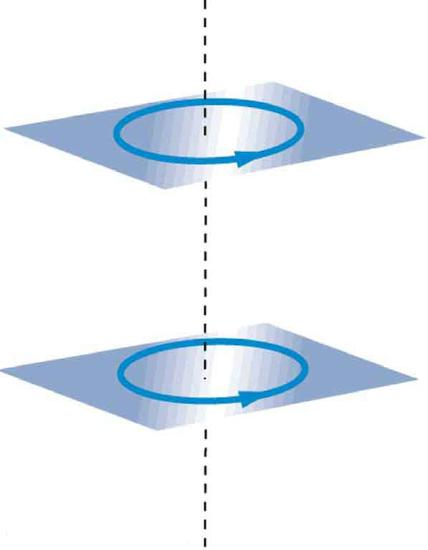
\includegraphics[scale=0.2]{loops}
		\end{center}
		\textbf{Answer} \\ \\
		When we use right hand rule we can see that the direction changes for current at each instant is on the same axis whether they are going in the same or opposite directions. We have seen in previous examples that there is a force of attraction when currents in opposite wires flow in the same direction and a force of repuslion when currents are in the opposite direction. You can show that by working out the direction of the magnetic fields of the wires.
		\question Calculate the magnetic field strength needed on a 200-turn square loop 40.0 cm on a side to create a maximum torque of $1600Nm$ if the loop is carrying 15.0 A.
		\textbf{Answer} \\ \\
		$$\mathcal{T}_{max}=NIAB\implies B=\dfrac{\mathcal{T}_{max}}{NIA}$$
		$$B=\dfrac{\mathcal{T}_{max}}{NIA}=\dfrac{1600Nm}{200\times15.0A\times(0.40m)^2}$$
		\begin{enumerate}[label=(\alph*)]
			\item At what angle is the current loop when the torque loop 80\% of the maximum?
			$$\mathcal{T}=NIAB\cos\theta\text{, such that the angle is between the area vector and the field}$$	
			$$\cos\theta=\dfrac{\mathcal{T}}{NIAB}\implies\cos\theta=\dfrac{\mathcal{T}}{\mathcal{T}_{max}}$$
			$$\cos\theta=0.8$$
			$$\theta=\arccos0.8$$
			\item What about 50\% of the maximum?
			$$\mathcal{T}=NIAB\cos\theta\text{, such that the angle is between the area vector and the field}$$	
			$$\cos\theta=\dfrac{\mathcal{T}}{NIAB}\implies\cos\theta=\dfrac{\mathcal{T}}{\mathcal{T}_{max}}$$
			$$\cos\theta=0.5$$
			$$\theta=\arccos0.5=\dfrac{\pi}{3}$$
		\end{enumerate}
		\question Why do we add a ferromagnetic material inside of a solenoid? What changes does it bring?
		\textbf{Answer} \\ \\
		A ferromagnetic core inside of a solenoid increases the premeablity of the solenoid which increases the magnetic field for the same amount of current. This makes solenoids more effective in inducing magnetic fields.
		\question The force on the rectangular loop of wire in the magnetic field in the figure below can be used to measure field strength. The field is uniform, and the plane of the loop is perpendicular to the field.
		\begin{center}
			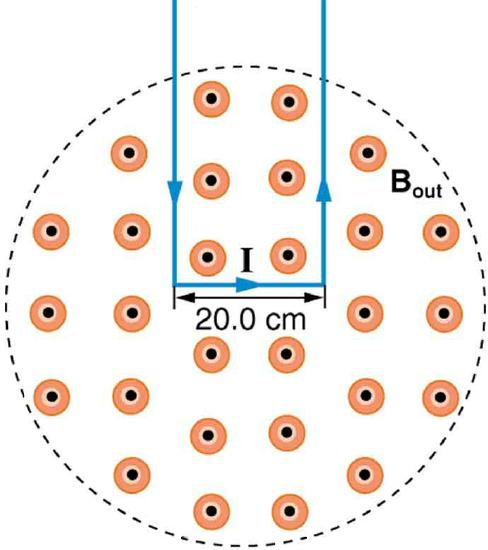
\includegraphics[scale=0.3]{loop1}
		\end{center}
		\begin{enumerate}[label=(\roman*)]
			\item What is the direction of the magnetic force on the loop?  \\ 
			\textbf{Answer} \\ \\
			The forces on the left and right sides of the loop cancel out, but the bottom side will have a force, so we only need to find the direction of the force on the bottom segment.
			$$\vec{F}=I\vec{l}\times\vec{B}$$
			$$\vec{F}=I\vec{l}\times\vec{B}$$
			$$\vec{F}=\hat{i}\times\hat{k}$$
			$$\vec{F}=-\hat{j}$$
			So the direction of the force on the loop is downwards.	
			\item If a current of 8.00 A is used, what is the force per unit magnetic field on the loop?
			$$F=ILB\sin\theta\text{ but }\sin\theta=1\text{ because }\vec{l}\perp\vec{B}$$
			$$\dfrac{F}{B}=IL$$
			$$\dfrac{F}{B}=8.00A\times0.2m$$
			$$\dfrac{F}{B}=4N/T$$
			\item What is the net torque on the loop?
			If the side length of the loop is l, the torque is approximately $\mathcal{T}=IBlw$.
			$\mathcal{T}=8.00A\times0.2m\times l\times B$
		\end{enumerate}
		\question Show that the Hall emf induced during the motion of a conductor in a perpendicular magnetic field is perpendicular to both the magnetic field and the velocity of the conductor. \\ \\
		We have seen that the emf induced during the Hall Effect is a result of the magnetic force, which is only present when the magnetic field has a component perpendicular to the velocity of the conductor. As the emf is induced, it is along the conductor which makes it perpendicular to both the field and the velocity.
		\subsection*{Advanced Problems}
		\question \begin{center}
			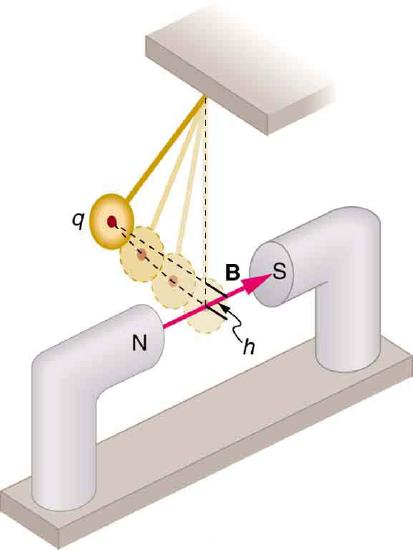
\includegraphics[scale=0.4]{pen}
		\end{center}
		\begin{enumerate}[label=(\alph*)]
			\item A pendulum is set up so that its bob swings between the poles of a permanent magnet as shown in the figure above. What is the magnitude and direction of the magnetic force on the bob at the lowest point in its path, if it has a positive $0.80\mu C$ charge and is released from a height of 25.0 cm above its lowest point? The magnetic field strength is 10.50 T.
			\item What is the acceleration of the bob at the bottom of its swing if its mass is 50.0 grams and is hung from a flexible string?
		\end{enumerate}
		\question One of the important applications of the magnetic force is in Magnetohydrodynamics. Discuss what it is and what its uses are.
		\question The Dutch (\textit{Nederlands}) for a Microwave is "Magnetron". Research and explain why the word magnetron makes sense.
	\end{questions}		
\end{document}